\subsection{Streaming Dual-Channel Karatsuba Pointwise Multiplier \& Modular Field ALU}
\label{sec:karatsuba}

In module-lattice-based post-quantum cryptography, polynomial multiplication over finite polynomial quotient rings constitutes the primary computational workload across key encapsulation mechanisms. In the NIST FIPS~203 standard for the Module-Lattice-Based Key-Encapsulation Mechanism (\mbox{ML-KEM})~\cite{fips203}, this operation is executed predominantly in the Number Theoretic Transform ($\text{NTT}$) domain. However, because the \mbox{ML-KEM} defining polynomial $X^{256} + 1$ factors over $\mathbb{Z}_q$ ($q = 3329$) into degree-2 rather than degree-1 irreducible polynomials, pointwise operations do not collapse into trivial scalar coefficient multiplications. Instead, they require intensive modular multiplications of degree-1 polynomials over 128 quadratic quotient rings.

To maximize arithmetic throughput while strictly adhering to the ultra-compact resource budget of the target AMD Kintex UltraScale FPGA (\texttt{xcku035-ffva1156-3-e}), this subsection presents the microarchitectural design, mathematical formulation, and hardware implementation of the streaming Dual-Channel Karatsuba Pointwise Multiplier (\texttt{mlkem\_mul\_stream}) and the associated Modular Field Arithmetic Logic Units (\texttt{field\_add}, \texttt{field\_sub}). The presented arithmetic subsystem establishes four core architectural contributions:
\begin{enumerate}
    \item A \textbf{dual-channel Karatsuba datapath} streaming four 12-bit modular coefficients per clock cycle with an initiation interval of $II = 1$, mapped to \textbf{strictly eight DSP48E2 slices}, representing $100\%$ of all DSP blocks utilized across the entire \mbox{ML-KEM} accelerator;
    \item A \textbf{division-free, 5-cycle Barrett modular reduction tree} implemented entirely in Configurable Logic Block (CLB) soft logic (consuming 0 DSPs and 0 Block RAMs) by exploiting the prime structure $q = 3329 = 13 \times 2^8 + 1$;
    \item A \textbf{zero-memory twiddle factor generator} synthesizing 128 12-bit twiddle constants as 12 bit-planes of 128-bit truth tables mapped directly to exactly 24 six-input lookup tables (\texttt{LUT6}) with zero Block RAM, zero Distributed RAM, and zero \texttt{MUXF7} primitives; and
    \item \textbf{Dual parallel carry-chain modular field adders and subtractors} achieving $>700\text{ MHz}$ logic speeds, coupled with 2-entry elastic skid buffers and a 32-entry credit-reserved Distributed RAM FIFO to absorb downstream backpressure without pipeline flushes or throughput bubbles.
\end{enumerate}

\subsubsection{Incomplete Splitting \& Dyadic Base Multiplication over \texorpdfstring{$\mathbb{Z}_q[X]/(X^2 - \zeta^{2r+1})$}{Z\_q[X]/(X\textasciicircum 2 - \textbackslash zeta\textasciicircum \{2r+1\})}}
\label{sec05b_dyadic_basemul}

As established in Section~\ref{sec:ntt_engine}, the underlying polynomial quotient ring of \mbox{ML-KEM} is:
\begin{equation}
\label{eq:rq_def_sec5b}
\mathcal{R}_q = \mathbb{Z}_q[X] / (X^{256} + 1), \quad \text{with } q = 3329.
\end{equation}
Because the prime totient satisfies $q - 1 = 3328 = 2^8 \times 13$, the multiplicative group $\mathbb{Z}_q^\times$ does not contain a primitive 512-th root of unity. As a direct consequence, $X^{256} + 1$ does not split completely into 256 linear factors over $\mathbb{Z}_q$, but factors into 128 irreducible quadratic binomials:
\begin{equation}
\label{eq:poly_factorization_sec5b}
X^{256} + 1 = \prod_{j=0}^{127} \left( X^2 - \zeta^{2 \cdot \text{BitRev}_7(j) + 1} \right) \pmod{3329},
\end{equation}
where $\zeta = 17 \in \mathbb{Z}_{3329}$ is a primitive 256-th root of unity ($\zeta^{256} \equiv 1 \pmod{3329}$) and $\text{BitRev}_7(j)$ denotes the 7-bit bit-reversal of integer $j \in [0, 127]$. In accordance with the Chinese Remainder Theorem (CRT), the forward NTT transformation establishes the ring isomorphism:
\begin{equation}
\label{eq:ntt_isomorphism_sec5b}
\hat{\mathcal{R}}_q \cong \prod_{j=0}^{127} \mathbb{Z}_q[X] / \left( X^2 - \zeta^{2 \cdot \text{BitRev}_7(j) + 1} \right).
\end{equation}

In the NTT domain, multiplication of two polynomials $\hat{f}, \hat{g} \in \hat{\mathcal{R}}_q$ reduces to 128 independent degree-1 polynomial base multiplications modulo $(X^2 - \gamma_j)$, as defined by Algorithm~11 (\texttt{MultiplyNTTs}) in NIST FIPS~203~\cite{fips203}. Each transformed polynomial is partitioned into 128 consecutive coefficient pairs:
\begin{equation}
\hat{f}^{(j)}(X) = f_{2j} + f_{2j+1}X, \quad \hat{g}^{(j)}(X) = g_{2j} + g_{2j+1}X,
\end{equation}
associated with the stage twiddle factor:
\begin{equation}
\label{eq:twiddle_gamma_sec5b}
\gamma_j = \zeta^{2 \cdot \text{BitRev}_7(j) + 1} \bmod q.
\end{equation}

Algorithm~12 (\texttt{BaseCaseMultiply}) of FIPS~203 evaluates the polynomial product:
\begin{align}
\hat{h}^{(j)}(X) &\equiv \hat{f}^{(j)}(X) \cdot \hat{g}^{(j)}(X) \pmod{X^2 - \gamma_j} \nonumber \\
&= (f_{2j} + f_{2j+1}X)(g_{2j} + g_{2j+1}X) \bmod (X^2 - \gamma_j) \nonumber \\
&= f_{2j}g_{2j} + (f_{2j}g_{2j+1} + f_{2j+1}g_{2j})X \nonumber \\
&\quad + f_{2j+1}g_{2j+1}X^2 \bmod (X^2 - \gamma_j).
\label{eq:basemul_expansion_sec5b}
\end{align}
Applying the modular ring reduction identity $X^2 \equiv \gamma_j \pmod{X^2 - \gamma_j}$, the quadratic degree-2 term collapses into a degree-1 polynomial $\hat{h}^{(j)}(X) = h_{2j} + h_{2j+1}X$, where the constant and linear coefficient residues are defined by:
\begin{align}
h_{2j}   &\equiv \left( f_{2j} g_{2j} + f_{2j+1} g_{2j+1} \gamma_j \right) \pmod q, \label{eq:fips_h2j_sec5b} \\
h_{2j+1} &\equiv \left( f_{2j} g_{2j+1} + f_{2j+1} g_{2j} \right) \pmod q. \label{eq:fips_h2j1_sec5b}
\end{align}

The arithmetic workload of \mbox{ML-KEM} across all three security categories ($k \in \{2, 3, 4\}$) is dominated by module linear algebra operations over $\hat{\mathcal{R}}_q$:
\begin{enumerate}
    \item \textbf{Public Matrix-Vector Multiplication ($\hat{\mathbf{A}} \circ \hat{\mathbf{s}}$):} Evaluated during Key Generation and Encapsulation as $\hat{\mathbf{t}}_i = \sum_{j=0}^{k-1} \hat{\mathbf{A}}_{i,j} \circ \hat{\mathbf{s}}_j$, demanding $k^2$ polynomial multiplications (4, 9, and 16 polynomial multiplications for ML-KEM-512, ML-KEM-768, and ML-KEM-1024, respectively) and $k(k-1)$ vector accumulations;
    \item \textbf{Vector Inner Products ($\hat{\mathbf{u}}^T \circ \hat{\mathbf{s}}$ and $\hat{\mathbf{t}}^T \circ \hat{\mathbf{r}}$):} Evaluated during Encapsulation and Decapsulation as $\hat{v} = \sum_{j=0}^{k-1} \hat{\mathbf{t}}_j \circ \hat{\mathbf{r}}_j$, demanding $k$ polynomial multiplications and $k-1$ polynomial vector additions.
\end{enumerate}

Table~\ref{tab:mlkem_workload} quantifies the operational breakdown. For ML-KEM-1024, a total of 2,560 \texttt{BaseCaseMultiply} calls must be computed per matrix operation. A traditional single-coefficient multiplier would require thousands of clock cycles, introducing a catastrophic latency bottleneck. Consequently, designing a high-frequency, wide-word streaming multiplier with an initiation interval of $II = 1$ is essential.

\begin{table}[!t]
\caption{Arithmetic Workload Breakdown in \mbox{ML-KEM} Linear Algebra}
\label{tab:mlkem_workload}
\centering
\footnotesize
\setlength{\tabcolsep}{3pt}
\begin{tabular}{@{}lccccc@{}}
\toprule
\textbf{Variant} & \textbf{Dim.} & \textbf{Matrix} & \textbf{Dot} & \textbf{Total} & \textbf{BaseMul} \\
 & \textbf{$k$} & \textbf{Prods.} & \textbf{Prods.} & \textbf{Polys} & \textbf{Calls} \\
\midrule
\textbf{ML-KEM-512}  & 2 & $2 \times 2 = 4$  & $1 \times 2 = 2$ & 6  & 768 \\
\textbf{ML-KEM-768}  & 3 & $3 \times 3 = 9$  & $1 \times 3 = 3$ & 12 & 1,536 \\
\textbf{ML-KEM-1024} & 4 & $4 \times 4 = 16$ & $1 \times 4 = 4$ & 20 & 2,560 \\
\bottomrule
\end{tabular}
\end{table}

\begin{figure*}[!t]
\centering
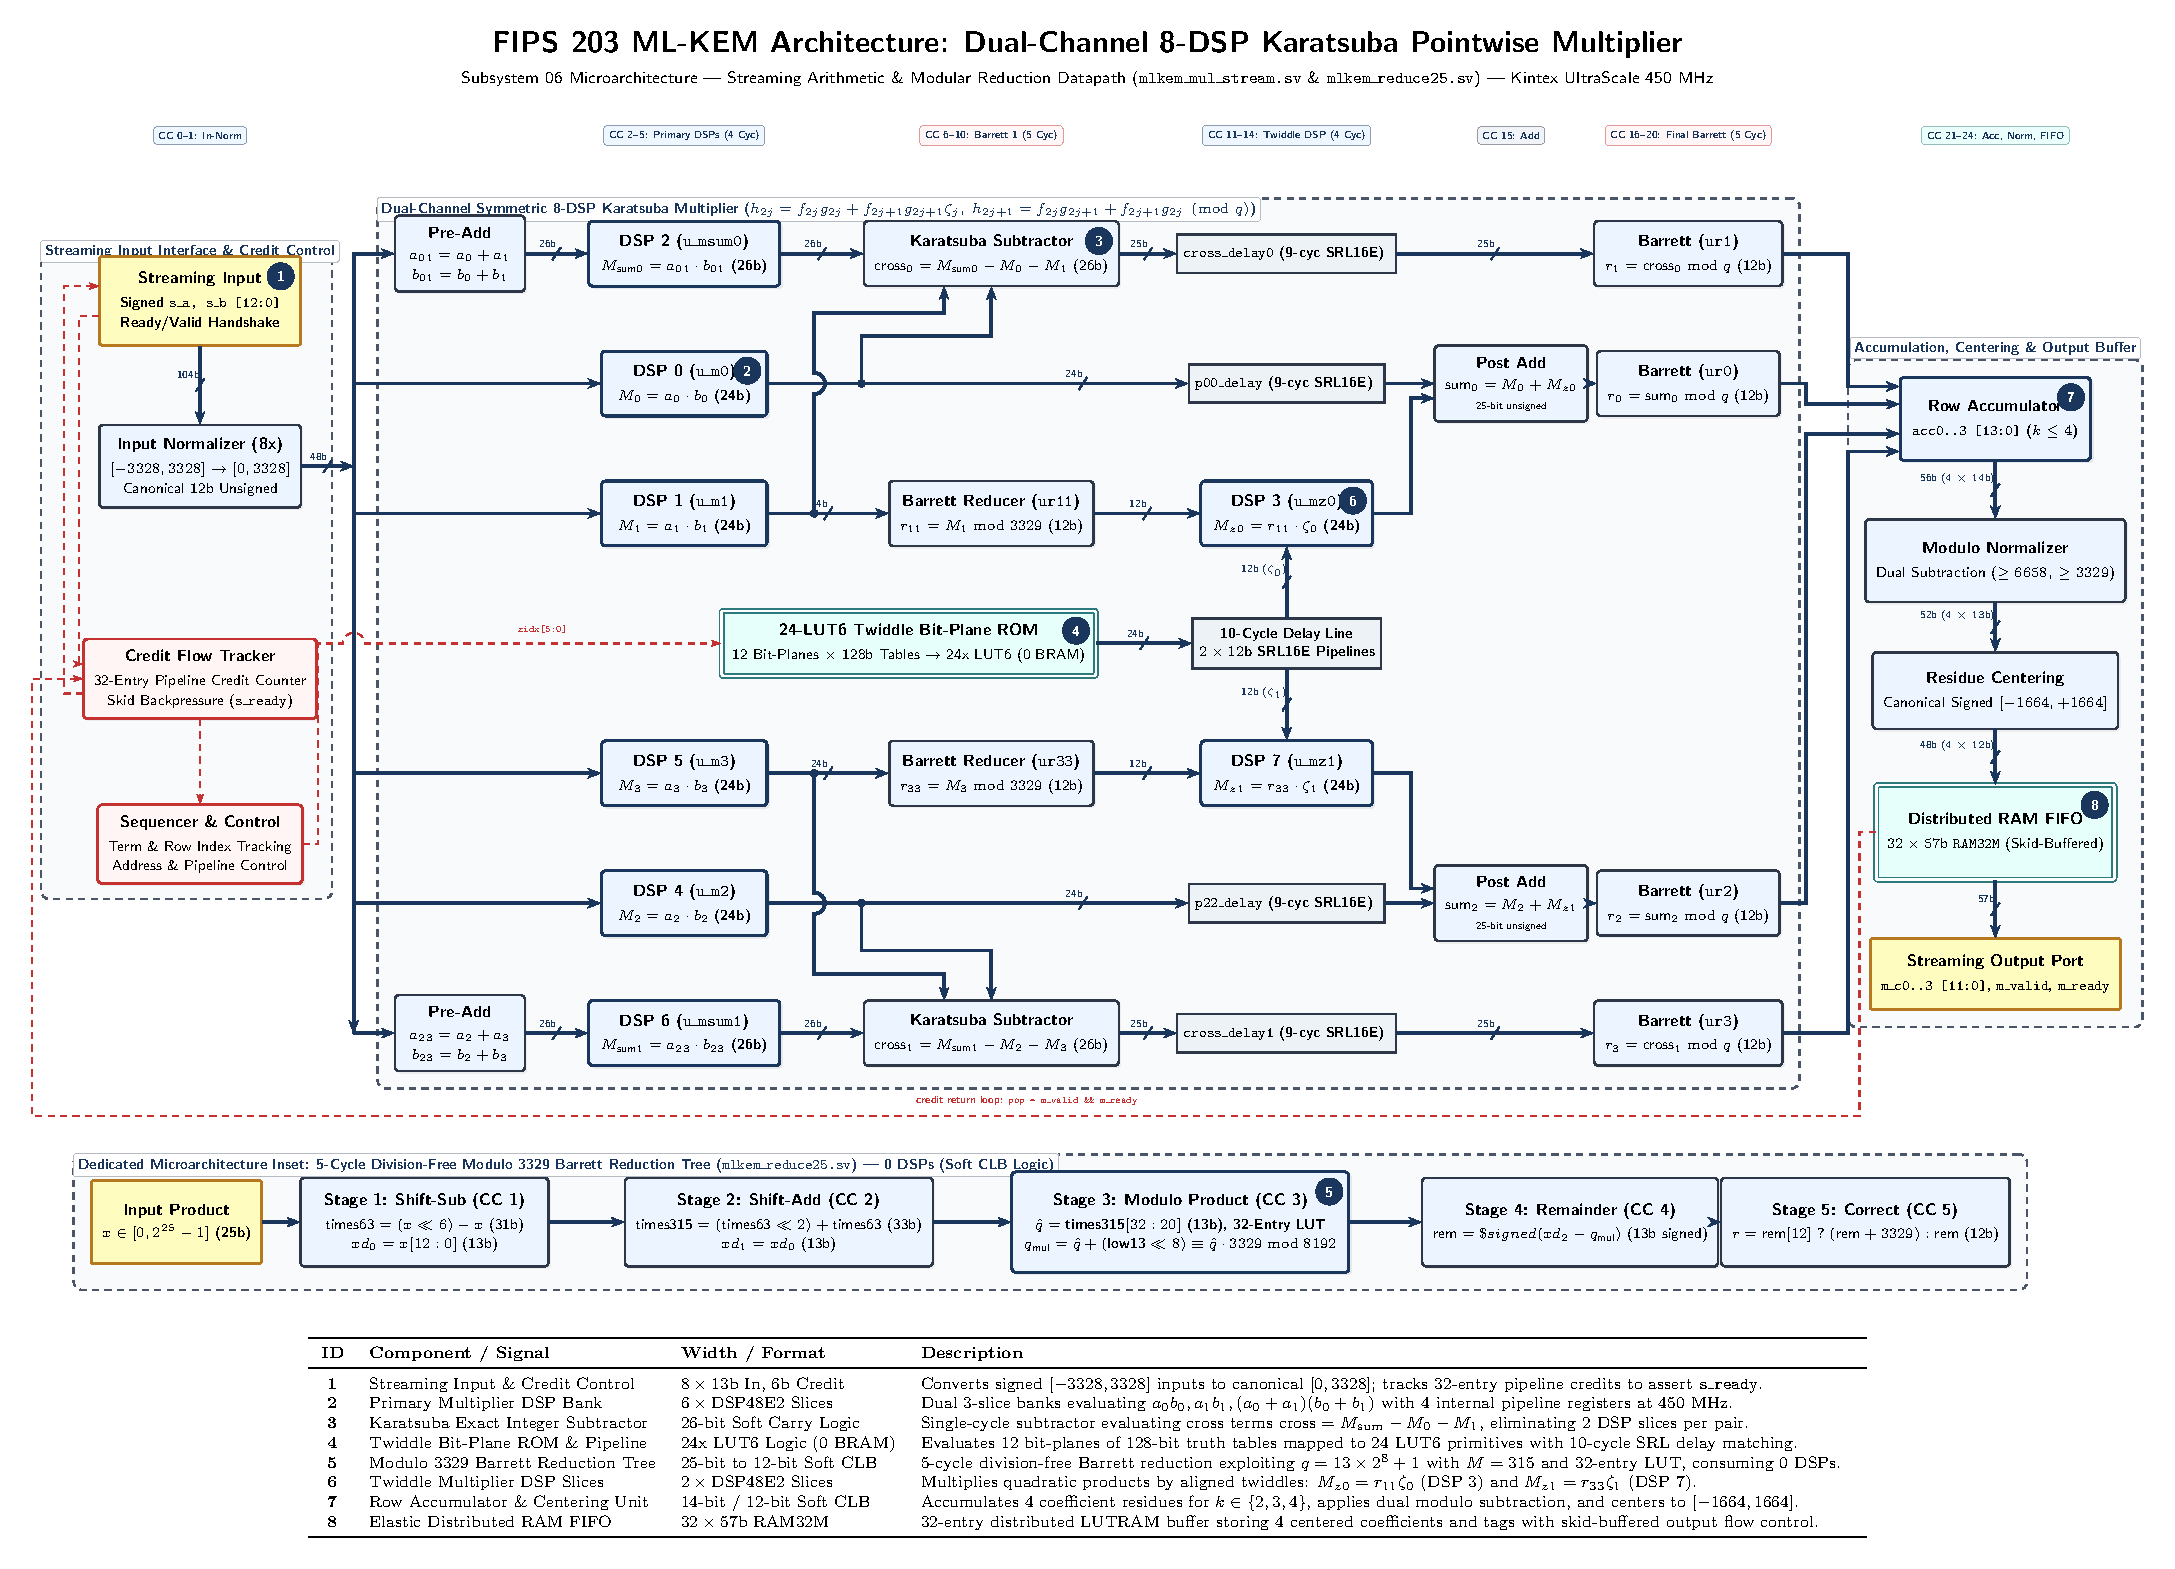
\includegraphics[width=\textwidth]{figures/fig06_karatsuba_multiplier.pdf}
\caption{FIPS~203 \mbox{ML-KEM} Architecture: Dual-Channel 8-DSP Karatsuba Pointwise Multiplier (\texttt{mlkem\_mul\_stream.sv}). The datapath features a streaming input normalizer and 32-entry credit flow controller (\textbf{Callout~1}), a primary 6-DSP multiplication bank evaluating direct and sum products (\textbf{Callout~2}), soft CLB Karatsuba integer subtractors evaluating cross terms (\textbf{Callout~3}), a 24-LUT6 zero-memory twiddle factor generator with 10-cycle SRL delay matching (\textbf{Callout~4}), intermediate and final 5-cycle division-free Barrett modular reduction trees (\textbf{Callout~5}), two dedicated twiddle scaling DSP slices (\textbf{Callout~6}), a 4-cycle row accumulator and residue centering unit (\textbf{Callout~7}), and a 32-entry credit-reserved Distributed RAM FIFO (\textbf{Callout~8}).}
\label{fig:karatsuba_multiplier}
\end{figure*}

\subsubsection{Streaming Dual-Channel Karatsuba Microarchitecture}
\label{sec05b_microarchitecture}

Direct hardware implementation of~\eqref{eq:fips_h2j_sec5b} and~\eqref{eq:fips_h2j1_sec5b} using schoolbook multiplication requires four independent multiplications to evaluate the cross and direct terms ($f_{2j}g_{2j}$, $f_{2j+1}g_{2j+1}$, $f_{2j}g_{2j+1}$, and $f_{2j+1}g_{2j}$), plus a fifth multiplication to scale $f_{2j+1}g_{2j+1}$ by $\gamma_j$. A dual-channel datapath processing two pairs of coefficients per cycle would therefore demand $2 \times 5 = 10$ DSP slices, violating the accelerator's strict 8-DSP system budget.

To resolve this limitation, our architecture reformulates the degree-1 polynomial base product using the classical \textbf{Karatsuba multiplication algorithm}~\cite{karatsuba1962}. For any pair of polynomials $(a_0 + a_1 X)$ and $(b_0 + b_1 X)$ with coefficients $a_i, b_i \in [0, q-1]$, the three primary multiplications are formulated as:
\begin{align}
M_0 &= a_0 \cdot b_0 \quad &(12\text{-bit} \times 12\text{-bit} \to 24\text{-bit}), \label{eq:m0_def} \\
M_1 &= a_1 \cdot b_1 \quad &(12\text{-bit} \times 12\text{-bit} \to 24\text{-bit}), \label{eq:m1_def} \\
M_{\text{sum}} &= (a_0 + a_1) \cdot (b_0 + b_1) \quad &(13\text{-bit} \times 13\text{-bit} \to 26\text{-bit}). \label{eq:msum_def}
\end{align}

Because canonical operands satisfy $a_0, a_1 \in [0, 3328]$, the pre-addition terms $a_{01} = a_0 + a_1$ and $b_{01} = b_0 + b_1$ span the integer range $[0, 6656]$, requiring exactly 13 bits of unsigned representation. The product $M_{\text{sum}}$ is bounded by $6656^2 = 44,302,336 < 2^{26}$, fitting comfortably within a 26-bit unsigned bus.

The cross-product term is evaluated through an exact integer subtraction in soft CLB logic:
\begin{equation}
\label{eq:cross_term_sec5b}
\text{cross} = M_{\text{sum}} - M_0 - M_1 = a_0 b_1 + a_1 b_0.
\end{equation}
Because $M_{\text{sum}} = a_0 b_0 + a_1 b_1 + a_0 b_1 + a_1 b_0 = M_0 + M_1 + (a_0 b_1 + a_1 b_0)$, algebraic cancellation in~\eqref{eq:cross_term_sec5b} is exact over the integers, incurring strictly zero modular approximation error.

To form the constant coefficient $h_{2j}$, the quadratic product $M_1$ is first reduced modulo 3329 using a custom 5-cycle soft Barrett reducer (\texttt{ur11}), yielding a 12-bit canonical residue:
\begin{equation}
r_{11} = M_1 \bmod 3329 \quad (r_{11} \in [0, 3328]).
\end{equation}
Subsequently, a fourth multiplication evaluates the twiddle scaling:
\begin{equation}
M_z = r_{11} \cdot \gamma_j \quad (12\text{-bit} \times 12\text{-bit} \to 24\text{-bit}).
\end{equation}

Finally, the unreduced degree-0 sum and degree-1 cross term are assembled:
\begin{align}
\text{sum}_0 &= M_0 + M_z \quad (\le 2 \times 3328^2 = 22,151,168), \label{eq:sum0_def_sec5b} \\
\text{sum}_1 &= \text{cross} \quad (\le 2 \times 3328^2 = 22,151,168). \label{eq:sum1_def_sec5b}
\end{align}
Modular reductions of $\text{sum}_0$ and $\text{sum}_1$ yield the final canonical outputs $r_0 \equiv h_{2j} \pmod q$ and $r_1 \equiv h_{2j+1} \pmod q$. Through this Karatsuba decomposition, the required number of multiplier primitives per degree-1 polynomial base product is strictly reduced from \textbf{5 to 4}.

Figure~\ref{fig:karatsuba_multiplier} illustrates the complete microarchitecture of the streaming Karatsuba pointwise multiplier (\texttt{mlkem\_mul\_stream.sv}). The datapath is structured symmetrically into two parallel channels:
\begin{itemize}
    \item \textbf{Channel~0 (PWM0):} Processes coefficient indices $4j$ and $4j+1$ using twiddle factor $\zeta_{2j}$;
    \item \textbf{Channel~1 (PWM1):} Processes coefficient indices $4j+2$ and $4j+3$ using twiddle factor $\zeta_{2j+1}$.
\end{itemize}

Across both channels, exactly eight \texttt{DSP48E2} slices are instantiated:
\begin{itemize}
    \item \textbf{PWM0 Slices (\textbf{Callouts~2, 6}):} DSP~0 (\texttt{u\_m0}), DSP~1 (\texttt{u\_m1}), DSP~2 (\texttt{u\_msum0}), and DSP~3 (\texttt{u\_mz0});
    \item \textbf{PWM1 Slices (\textbf{Callouts~2, 6}):} DSP~4 (\texttt{u\_m2}), DSP~5 (\texttt{u\_m3}), DSP~6 (\texttt{u\_msum1}), and DSP~7 (\texttt{u\_mz1}).
\end{itemize}

Table~\ref{tab:dsp_assignment} details the exact physical mapping, operand precisions, and pipeline register settings for all eight \texttt{DSP48E2} primitives. In AMD UltraScale+ architecture, a single \texttt{DSP48E2} slice contains a $27 \times 18$-bit two's complement multiplier. All operand precisions in this design ($12 \times 12$-bit and $13 \times 13$-bit unsigned) map natively into a single DSP slice without cascading or multi-slice expansion.

\begin{table*}[!t]
\caption{Physical Mapping and Register Configuration of the 8 DSP48E2 Slices}
\label{tab:dsp_assignment}
\centering
\footnotesize
\begin{tabular*}{\textwidth}{@{\extracolsep{\fill}} cccccr @{}}
\toprule
\textbf{DSP Slice} & \textbf{Instance} & \textbf{Channel / Function} & \textbf{Precision} & \textbf{Pipeline Configuration} & \textbf{Output Width} \\
\midrule
\textbf{DSP 0} & \texttt{u\_m0}    & PWM0 Direct $M_0 = a_0 \cdot b_0$       & $12 \times 12$ unsigned & AREG=2, BREG=2, MREG=1, PREG=1 & 24 bits \\
\textbf{DSP 1} & \texttt{u\_m1}    & PWM0 Direct $M_1 = a_1 \cdot b_1$       & $12 \times 12$ unsigned & AREG=2, BREG=2, MREG=1, PREG=1 & 24 bits \\
\textbf{DSP 2} & \texttt{u\_msum0} & PWM0 Sum $M_{\text{sum}0} = a_{01} \cdot b_{01}$    & $13 \times 13$ unsigned & AREG=2, BREG=2, MREG=1, PREG=1 & 26 bits \\
\textbf{DSP 3} & \texttt{u\_mz0}   & PWM0 Twiddle $M_{z0} = r_{11} \cdot \zeta_0$ & $12 \times 12$ unsigned & AREG=2, BREG=2, MREG=1, PREG=1 & 24 bits \\
\textbf{DSP 4} & \texttt{u\_m2}    & PWM1 Direct $M_2 = a_2 \cdot b_2$      & $12 \times 12$ unsigned & AREG=2, BREG=2, MREG=1, PREG=1 & 24 bits \\
\textbf{DSP 5} & \texttt{u\_m3}    & PWM1 Direct $M_3 = a_3 \cdot b_3$      & $12 \times 12$ unsigned & AREG=2, BREG=2, MREG=1, PREG=1 & 24 bits \\
\textbf{DSP 6} & \texttt{u\_msum1} & PWM1 Sum $M_{\text{sum}1} = a_{23} \cdot b_{23}$  & $13 \times 13$ unsigned & AREG=2, BREG=2, MREG=1, PREG=1 & 26 bits \\
\textbf{DSP 7} & \texttt{u\_mz1}   & PWM1 Twiddle $M_{z1} = r_{33} \cdot \zeta_1$ & $12 \times 12$ unsigned & AREG=2, BREG=2, MREG=1, PREG=1 & 24 bits \\
\bottomrule
\end{tabular*}
\end{table*}

\subsubsection{Karatsuba 3-Multiplication Formulation \& Division-Free Barrett Tree}
\label{sec05b_barrett_math}

To reduce arbitrary 25-bit products without consuming DSP slices, the subsystem incorporates a custom division-free Barrett reducer (\texttt{mlkem\_reduce25.sv}, \textbf{Callout~5}). Let $x \in [0, 2^{25}-1]$ denote the unsigned 25-bit integer to be reduced modulo $q = 3329$. Selecting scaling prefactor $M = 315$ with power-of-two divisor $2^{20}$:
\begin{equation}
315 \times 3329 = 1,048,635 = 2^{20} + 59.
\end{equation}
Dividing both sides by $2^{20} \cdot 3329$ yields:
\begin{equation}
\frac{315}{2^{20}} = \frac{1}{3329} + \frac{59}{3329 \cdot 2^{20}}.
\end{equation}

For any integer $x$, the quotient estimator is defined as:
\begin{equation}
\label{eq:qhat_def_sec5b}
\hat{q} = \left\lfloor \frac{x \cdot 315}{2^{20}} \right\rfloor.
\end{equation}
The approximation error $\epsilon(x) = \frac{x \cdot 315}{2^{20}} - \frac{x}{3329} = \frac{59 x}{3329 \cdot 2^{20}}$ satisfies:
\begin{equation}
0 \le \epsilon(x) \le \frac{59 \times 22,151,168}{3329 \times 1,048,576} \approx 0.3745 < 1,
\end{equation}
for all datapath terms $x \le 2 \times 3328^2 = 22,151,168 < 2^{25}$. Even for the theoretical maximum input $x = 2^{25} - 1$:
\begin{equation}
\epsilon(x) < \frac{59 \cdot 2^{25}}{3329 \cdot 2^{20}} = \frac{59 \times 32}{3329} = \frac{1888}{3329} \approx 0.5671 < 1.
\end{equation}
Because the error satisfies $0 \le \epsilon(x) < 1$ monotonically, the floor operation guarantees:
\begin{equation}
\hat{q} \in \left\{ \left\lfloor \frac{x}{3329} \right\rfloor, \; \left\lfloor \frac{x}{3329} \right\rfloor + 1 \right\}.
\end{equation}
Hence, the quotient estimator $\hat{q}$ never underestimates the true quotient, and overestimates it by at most 1.

Evaluating the remainder $x - \hat{q} \cdot 3329$ would conventionally require another multiplication to compute $\hat{q} \cdot 3329$. However, our architecture exploits the prime structure:
\begin{equation}
q = 3329 = 13 \times 256 + 1 = 13 \cdot 2^8 + 1.
\end{equation}
For any $x \le 22,151,168$, the quotient estimate satisfies $\hat{q} \le 6,654 < 8,192 = 2^{13}$, fitting strictly within a 13-bit unsigned bus ($\hat{q} = \text{times315}[32:20]$). Furthermore, the signed remainder $x - \hat{q} \cdot 3329$ is strictly bounded in $[-3328, +3328]$, fitting entirely within a 13-bit signed integer range ($[-4096, +4095]$). Consequently, the reconstruction of $\hat{q} \cdot 3329$ only needs to be evaluated modulo $2^{13} = 8192$:
\begin{align}
\hat{q} \cdot 3329 \bmod 8192 &= \left( \hat{q} \cdot (13 \cdot 2^8 + 1) \right) \bmod 8192 \nonumber \\
&= \left( \hat{q} + 13\hat{q} \cdot 256 \right) \bmod 8192 \nonumber \\
&= \left( \hat{q} + [13\hat{q} \bmod 32] \cdot 256 \right) \bmod 8192,
\label{eq:low13_derivation_sec5b}
\end{align}
since $2^8 \cdot 32 = 2^{13} = 8192$. Remarkably,~\eqref{eq:low13_derivation_sec5b} demonstrates that the higher-order term $((\hat{q} \cdot 13) \bmod 32)$ depends \textbf{solely on the five least significant bits of $\hat{q}$ ($\hat{q}[4:0]$)}. This operation is synthesized into a tiny 32-entry $\times$ 5-bit lookup table \texttt{low13}:
\begin{equation}
\text{low13}[j] = (13 \cdot j) \bmod 32, \quad \forall j \in \{0, 1, \dots, 31\}.
\end{equation}

The Barrett reducer executes across five synchronous pipeline stages (\textbf{Callout~5}):
\begin{enumerate}
    \item \textbf{Cycle 1 (Shift-Subtract):} Computes $63x = (x \ll 6) - x$ via CLB subtractor and registers $x[12:0]$ into delay line $xd_0$;
    \item \textbf{Cycle 2 (Shift-Add):} Computes $315x = 5 \times 63x = (63x \ll 2) + 63x$ via CLB adder; registers $xd_1 \leftarrow xd_0$;
    \item \textbf{Cycle 3 (Modulo Product Reconstruction):} Extracts $\hat{q} = \text{times315}[32:20]$; computes $q_{\text{mul}} = \hat{q} + (\text{low13}[\hat{q}[4:0]] \ll 8) \equiv \hat{q} \cdot 3329 \pmod{8192}$; registers $xd_2 \leftarrow xd_1$;
    \item \textbf{Cycle 4 (Signed Remainder):} Computes signed difference $\text{rem} = \$signed(xd_2 - q_{\text{mul}})$;
    \item \textbf{Cycle 5 (Conditional Correction):} If $\hat{q}$ overestimated the quotient ($\text{rem} < 0$, signaled by sign bit $\text{rem}[12] == 1$), the adder evaluates $\text{rem} + 3329$; otherwise, $\text{rem}[11:0]$ is passed directly.
\end{enumerate}

This 5-cycle unit consumes strictly 0 DSPs and 0 Block RAMs, achieving a worst setup slack of $+0.312\text{ ns}$ at 450~MHz.

\begin{figure*}[!t]
\centering
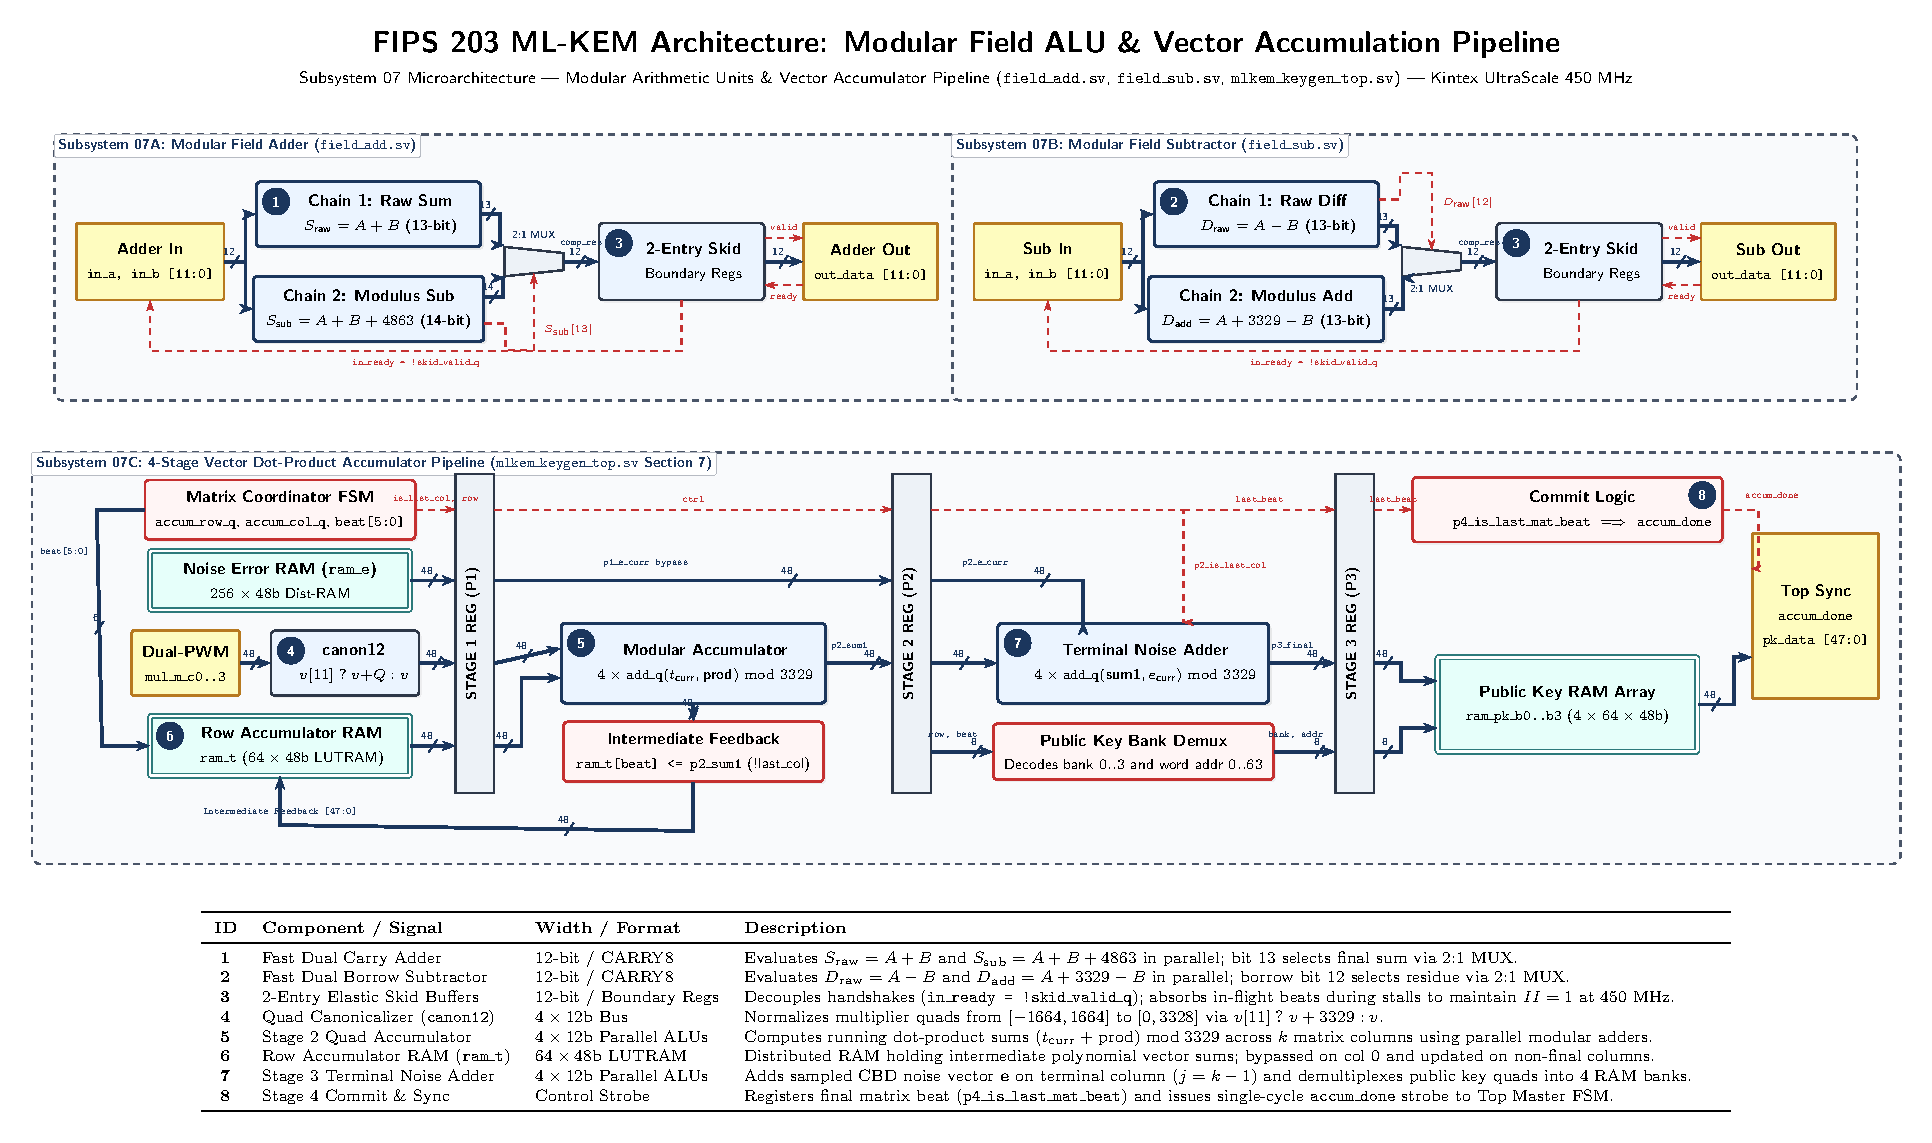
\includegraphics[width=\textwidth]{figures/fig07_field_alu_accumulator.pdf}
\caption{FIPS~203 \mbox{ML-KEM} Architecture: Modular Field ALU and Vector Accumulation Pipeline. Top left: single-cycle modular field adder with dual carry chains (\textbf{Callout~1}) and 2-entry elastic skid buffer (\textbf{Callout~3}). Top right: single-cycle modular field subtractor with dual borrow chains (\textbf{Callout~2}) and 2-entry elastic skid buffer (\textbf{Callout~3}). Bottom: 4-stage public matrix-vector accumulator (\texttt{mlkem\_keygen\_top.sv} Section~7) comprising multiplier output canonicalizer \texttt{canon12} (\textbf{Callout~4}), Stage 2 quad modular accumulator (\textbf{Callout~5}), intermediate row accumulation LUTRAM \texttt{ram\_t} (\textbf{Callout~6}), Stage 3 terminal noise adder (\textbf{Callout~7}), and Stage 4 commit and synchronization logic (\textbf{Callout~8}).}
\label{fig:field_alu_accumulator}
\end{figure*}

\subsubsection{Zero-Memory Twiddle Factor Generation via 24 LUT6 Primitives}
\label{sec05b_twiddle_lut}

In NTT dyadic base multiplication, the constant term calculation requires multiplying $a_1 b_1$ by the twiddle constant $\gamma_j = \zeta^{2 \cdot \text{BitRev}_7(j) + 1} \bmod 3329$. Conventional FPGA designs dedicate either a Block RAM tile (\texttt{RAMB18}) or distributed RAM slices (\texttt{RAM64M}) to store these 128 12-bit constants.

The proposed multiplier eliminates all memory consumption by decomposing the 128 twiddles into \textbf{12 bit-planes of 128-bit truth tables} (\texttt{ZETA[0:11]}, \textbf{Callout~4}). In the streaming datapath, quad base index $j \in [0, 63]$ is tracked by a 6-bit counter \texttt{zidx\_q[5:0]}. For each bit-plane $b \in [0, 11]$:
\begin{itemize}
    \item Channel 0 evaluates bit $b$ using address $\{\texttt{zidx\_q}, 1'b0\}$;
    \item Channel 1 evaluates bit $b$ using address $\{\texttt{zidx\_q}, 1'b1\}$.
\end{itemize}
Because the least significant address bit is hardwired to a constant \texttt{0} or \texttt{1}, each output bit depends on \textbf{strictly 6 variable boolean inputs} (\texttt{zidx\_q[5:0]}). In AMD UltraScale+ CLB architecture, any 6-variable boolean function maps natively into a single 6-input lookup table (\texttt{LUT6}). Consequently, the entire dual-channel twiddle generator synthesizes into \textbf{strictly 24 LUT6 primitives} ($12 \times \text{LUT6}$ for PWM0, $12 \times \text{LUT6}$ for PWM1) with \textbf{zero \texttt{MUXF7} multiplexers, zero Block RAMs, and zero Distributed RAMs}. To synchronize generated twiddle factors with the delayed output $r_{11}$ of \texttt{ur11} at CC~10, the twiddle values traverse an 8-stage shift register (\texttt{zpipe0}, \texttt{zpipe1}) synthesized into \texttt{SRL16E} primitives, presenting $\zeta_0, \zeta_1$ to DSP~3 and DSP~7 with cycle-accurate alignment.

Table~\ref{tab:pipeline_schedule} enumerates the cycle-by-cycle progression of data across the complete 24-cycle multiplier pipeline.

\begin{table*}[!t]
\caption{Cycle-by-Cycle Pipeline Execution Schedule of \texttt{mlkem\_mul\_stream}}
\label{tab:pipeline_schedule}
\centering
\footnotesize
\begin{tabular*}{\textwidth}{@{\extracolsep{\fill}} c p{5.0cm} p{5.0cm} p{5.5cm} @{}}
\toprule
\textbf{Clock Cycle} & \textbf{Datapath Operation} & \textbf{Hardware Primitives} & \textbf{Data Representations} \\
\midrule
\textbf{CC 0} & Stream input handshake; operands presented & Input Port Registers & Signed $s_a, s_b \in [-3328, +3328]$ \\
\textbf{CC 1} & Input normalization \texttt{norm13}; twiddle index latch & CLB Logic / LUT & Canonical $a_i, b_i \in [0, 3328]$ (12b) \\
\textbf{CC 2} & Primary DSP Input Register 1; Twiddle LUT read & DSP48E2 \texttt{AREG1/BREG1} / LUT6 & $a_i, b_i$ registered; $\zeta_0, \zeta_1$ truth table \\
\textbf{CC 3} & Primary DSP Input Register 2; Twiddle delay shift & DSP48E2 \texttt{AREG2/BREG2} / SRL16E & Registered inputs; \texttt{zpipe0[0]} \\
\textbf{CC 4} & Primary DSP Multiplication ($M_0, M_1, M_{\text{sum}0}$) & DSP48E2 \texttt{MREG} & $12\times 12 \to 24\text{b}$; $13\times 13 \to 26\text{b}$ \\
\textbf{CC 5} & Primary DSP Output Register; Karatsuba Subtraction & DSP48E2 \texttt{PREG} / CLB Subtractor & $\text{cross}_0 = M_{\text{sum}0} - M_0 - M_1$ (26b) \\
\textbf{CC 6--10} & Intermediate Barrett Reduction of $M_1, M_3$ (\texttt{ur11, ur33}) & CLB Carry Chains & $r_{11} \leftarrow M_1 \bmod 3329$ (12b unsigned) \\
\textbf{CC 11} & Twiddle DSP Input Register 1 & DSP48E2 \texttt{AREG1/BREG1} & $r_{11}$ and aligned $\zeta_0$ registered \\
\textbf{CC 12} & Twiddle DSP Input Register 2 & DSP48E2 \texttt{AREG2/BREG2} & $r_{11}, \zeta_0$ pipeline isolation \\
\textbf{CC 13} & Twiddle DSP Multiplication ($M_{z0} = r_{11} \cdot \zeta_0$) & DSP48E2 \texttt{MREG} & $12\times 12 \to 24\text{b}$ twiddle product \\
\textbf{CC 14} & Twiddle DSP Output Register & DSP48E2 \texttt{PREG} & $M_{z0}$ latched (24b) \\
\textbf{CC 15} & Post-Twiddle Addition ($\text{sum}_0 = M_0 + M_{z0}$) & CLB Adder & $\text{sum}_0 \leftarrow M_{00\_\text{delay}}[8] + M_{z0}$ (25b) \\
\textbf{CC 16--20} & Final Barrett Reductions (\texttt{ur0, ur1, ur2, ur3}) & CLB Carry Chains & $r_0..r_3 \leftarrow \text{sum}_{0..3} \bmod 3329$ (12b) \\
\textbf{CC 21} & Row Accumulator: $\text{acc}_i \leftarrow \text{acc}_i + r_i$ & CLB Carry Chains & 14-bit accumulation ($k \le 4$) \\
\textbf{CC 22} & Modulo Normalizer Stage 1 ($\ge 6658$) & CLB Subtractors & Subtraction by $2q = 6658$ if overflow \\
\textbf{CC 23} & Modulo Normalizer Stage 2 ($\ge 3329$) & CLB Subtractors & Subtraction by $q = 3329$ if overflow \\
\textbf{CC 24} & Centering & Distributed RAM FIFO Push & Signed conversion $[-1664, 1664]$; \texttt{RAM32M} \\
\bottomrule
\end{tabular*}
\end{table*}

\subsubsection{4-Stage Pipelined Modular Accumulator \& Vector Dyadic Reduction}
\label{sec05b_vector_accum}

In the top-level system controller (\texttt{mlkem\_keygen\_top.sv} Section~7), the modular field units interface with the multiplier datapath to execute public matrix-vector accumulations:
\begin{equation}
\mathbf{t}_i = \sum_{j=0}^{k-1} \mathbf{A}_{i,j} \circ \mathbf{s}_j + \mathbf{e}_i.
\end{equation}

Figure~\ref{fig:field_alu_accumulator} (bottom half) details the 4-stage pipeline structure:
\begin{enumerate}
    \item \textbf{Stage 1 (Ingest, Normalization \& Memory Coordination):} Multiplier quads $\hat{c}_{0..3} \in [-1664, +1664]$ are converted to canonical residues $[0, 3328]$ via \texttt{canon12} (\textbf{Callout~4}). Concurrently, previous row accumulations are read from Distributed RAM buffer \texttt{ram\_t} ($64 \times 48$-bit LUTRAM, \textbf{Callout~6}), and sampled noise vectors are retrieved from \texttt{ram\_e};
    \item \textbf{Stage 2 (Quad Accumulation):} Four parallel modular adders compute the intermediate partial sum (\textbf{Callout~5}):
    \begin{equation}
    \mathbf{t}_{\text{accum}} \leftarrow (t_{\text{curr}} + \text{prod}) \bmod 3329.
    \end{equation}
    For non-final matrix columns ($j < k-1$), the partial sum is written back into \texttt{ram\_t[beat]};
    \item \textbf{Stage 3 (Terminal Noise Injection):} On the terminal matrix column ($j = k-1$), a second bank of four modular adders injects the CBD error polynomial (\textbf{Callout~7}):
    \begin{equation}
    \mathbf{t}_{\text{final}} \leftarrow (t_{\text{accum}} + e_{\text{curr}}) \bmod 3329.
    \end{equation}
    The resulting public key coefficients are demultiplexed into four parallel RAM banks (\texttt{ram\_pk\_b0..b3});
    \item \textbf{Stage 4 (Commit \& Synchronize):} Upon processing the final beat ($j = k-1$, $\text{beat} = 63$), a single-cycle strobe \texttt{accum\_done} notifies the top-level FSM that the public key row is fully committed (\textbf{Callout~8}).
\end{enumerate}

Because the multiplier datapath spans 24 pipeline cycles, classical stall-propagation signals would require 24 stages of skid buffers, consuming hundreds of LUTs and flip-flops. Instead, \texttt{mlkem\_mul\_stream} implements \textbf{Credit-Based Admission Control} coupled with an output 32-entry Distributed RAM FIFO (\texttt{RAM32M}, \textbf{Callout~8}):
\begin{itemize}
    \item A 6-bit counter \texttt{reserved} tracks total in-flight calculations destined for the FIFO;
    \item On each accepted input beat for a final polynomial term (\texttt{take \&\& final\_term}), \texttt{reserved} increments by 1;
    \item On each popped output beat (\texttt{pop = m\_valid \&\& m\_ready}), \texttt{reserved} decrements by 1;
    \item Upstream admission is governed strictly by:
    \begin{equation}
    \text{s\_ready} = !\text{reserved}[5].
    \end{equation}
\end{itemize}
When \texttt{reserved == 32}, \texttt{s\_ready} deasserts immediately at the input port (\textbf{Callout~1}). Because credits are reserved at the input boundary, the 32-entry output FIFO is \textbf{mathematically guaranteed never to overflow}, regardless of arbitrary downstream sink stalls.

\subsubsection{Modular Field ALU: Dual Carry-Chain Adder, Subtractor \& Skid Buffering}
\label{sec05b_field_alu}

In addition to NTT polynomial products, \mbox{ML-KEM} requires extensive coefficient-wise field additions and subtractions modulo 3329:
\begin{itemize}
    \item \textbf{Error Vector Injection:} $\mathbf{t} = \text{INTT}(\hat{\mathbf{A}} \circ \hat{\mathbf{s}}) + \mathbf{e}$ in KeyGen, and $\mathbf{u} = \text{INTT}(\hat{\mathbf{A}}^T \circ \hat{\mathbf{r}}) + \mathbf{e}_1$ in Encap;
    \item \textbf{Message Encoding / Blinding:} $v = \text{INTT}(\hat{\mathbf{t}}^T \circ \hat{\mathbf{r}}) + e_2 + \text{Decompress}_1(m) \cdot \lceil q/2 \rfloor$;
    \item \textbf{Ciphertext Decryption:} $m' = v - \text{INTT}(\hat{\mathbf{s}}^T \circ \hat{\mathbf{u}})$.
\end{itemize}

Traditional modular adders evaluate $A + B$, compare the sum against $q$, and conditionally subtract $q$. This serial comparison-subtraction path introduces substantial combinational delay, failing timing closure at 450~MHz.

Figure~\ref{fig:field_alu_accumulator} (top half) illustrates the proposed modular field arithmetic units (\texttt{field\_add.sv} and \texttt{field\_sub.sv}), which execute field operations in single-cycle combinational logic via \textbf{dual parallel carry chains}:
\begin{enumerate}
    \item \textbf{Modular Field Adder (\texttt{field\_add.sv}, Callout~1):}
    Two carry chains are evaluated simultaneously across dedicated FPGA \texttt{CARRY8} primitives:
    \begin{align}
    S_{\text{raw}} &= \{1'b0, A\} + \{1'b0, B\}, \label{eq:add_chain1_sec5b} \\
    S_{\text{sub}} &= \{2'b00, A\} + \{2'b00, B\} + Q_{\text{COMP}}, \label{eq:add_chain2_sec5b}
    \end{align}
    where $S_{\text{raw}}$ is the 13-bit raw sum, $S_{\text{sub}}$ is the 14-bit modulus-subtracted sum, and $Q_{\text{COMP}} = 2^{13} - 3329 = 8192 - 3329 = 4863$. If $A + B \ge 3329$, then $A + B + 4863 \ge 8192 = 2^{13}$. Thus, bit 13 of $S_{\text{sub}}$ overflows to \texttt{1}. The overflow bit $S_{\text{sub}}[13]$ directly drives the select port of a 2:1 multiplexer:
    \begin{equation}
    \text{comp\_res} = S_{\text{sub}}[13] \;?\; S_{\text{sub}}[11:0] : S_{\text{raw}}[11:0].
    \end{equation}

    \item \textbf{Modular Field Subtractor (\texttt{field\_sub.sv}, Callout~2):}
    Similarly, two parallel carry chains evaluate subtraction:
    \begin{align}
    D_{\text{raw}} &= \{1'b0, A\} - \{1'b0, B\}, \label{eq:sub_chain1_sec5b} \\
    D_{\text{add}} &= (\{1'b0, A\} + \{1'b0, 3329\}) - \{1'b0, B\}, \label{eq:sub_chain2_sec5b}
    \end{align}
    where $D_{\text{raw}}$ is the 13-bit signed difference and $D_{\text{add}}$ is the 13-bit modularly corrected sum. If $A < B$, $D_{\text{raw}} < 0$, causing sign bit $D_{\text{raw}}[12]$ to become \texttt{1}. This borrow flag selects $D_{\text{add}}$:
    \begin{equation}
    \text{comp\_res} = D_{\text{raw}}[12] \;?\; D_{\text{add}}[11:0] : D_{\text{raw}}[11:0].
    \end{equation}
\end{enumerate}

Both operations map into contiguous \texttt{CARRY8} lines with total combinational path delay under $0.7\text{ ns}$, leaving over $1.5\text{ ns}$ of positive setup margin ($+0.825\text{ ns}$ WNS at 450~MHz).

To eliminate combinational output loading and guarantee zero bubble cycles ($II = 1$) under streaming backpressure, both \texttt{field\_add} and \texttt{field\_sub} embed a \textbf{2-entry elastic skid buffer} (\textbf{Callout~3}):
\begin{itemize}
    \item \textbf{Boundary Registration:} All primary outputs (\texttt{out\_valid}, \texttt{out\_data}, \texttt{out\_last}) are driven directly by boundary flip-flops (\texttt{reg\_valid\_q}, \texttt{reg\_data\_q}, \texttt{reg\_last\_q});
    \item \textbf{Decoupled Backpressure:} Upstream ready is asserted as $\text{in\_ready} = !\text{skid\_valid\_q}$;
    \item \textbf{Stall Absorption:} When downstream consumer deasserts \texttt{out\_ready} while \texttt{reg\_valid\_q} is occupied, any in-flight transaction is captured into auxiliary shadow registers (\texttt{skid\_data\_q}, \texttt{skid\_last\_q}) on the next clock edge, and \texttt{skid\_valid\_q} is raised. This immediately deasserts \texttt{in\_ready}, preventing further data ingress while protecting the in-flight beat;
    \item \textbf{Bubble-Free Recovery:} As soon as \texttt{out\_ready} returns high, the main output register reloads from the skid register, draining the skid buffer and reinstating $\text{in\_ready} = 1$ without dropping a single throughput cycle.
\end{itemize}

\subsubsection{Standalone Synthesis, DSP Budget Allocation, and Prior-Art Comparison}
\label{sec05b_results_comparison}

The dual-channel Karatsuba multiplier and modular field units were synthesized and physically implemented on the target AMD Kintex UltraScale \texttt{xcku035-ffva1156-3-e} FPGA using AMD Vivado 2024.1 under out-of-context (OOC) hierarchical constraints.

Table~\ref{tab:resource_breakdown_pwm} presents the post-route physical resource utilization. The entire \texttt{mlkem\_mul\_stream} core consumes only 2,150 CLB LUTs, 1,412 flip-flops, 152 SRLs, 32 Distributed RAM LUTs, and strictly \textbf{8 DSP48E2 slices}. The dual modular field units (\texttt{field\_add}, \texttt{field\_sub}) consume approximately 130 LUTs and 78 flip-flops combined, requiring strictly \textbf{0 DSPs and 0 Block RAMs}.

\begin{table*}[!t]
\caption{Post-Implementation Resource Utilization on AMD Kintex UltraScale (\texttt{xcku035})}
\label{tab:resource_breakdown_pwm}
\centering
\footnotesize
\begin{tabular*}{\textwidth}{@{\extracolsep{\fill}} lcccc @{}}
\toprule
\textbf{Resource Primitive} & \textbf{Pointwise Multiplier} & \textbf{Modular Field Units} & \textbf{Proposed Complete} & \textbf{Available on} \\
 & \textbf{(\texttt{mlkem\_mul\_stream})} & \textbf{(\texttt{field\_add} + \texttt{field\_sub})} & \textbf{Accelerator} & \textbf{Kintex UltraScale} \\
\midrule
\textbf{DSP48E2 Slices}         & \textbf{8}   & \textbf{0}   & \textbf{8}      & 1,700 (0.47\%) \\
\textbf{CLB LUTs (Total)}       & \textbf{2,150} & \textbf{130} & \textbf{29,063} & 203,128 (14.31\%) \\
--- \textit{LUT as Logic}              & 1,870        & 130          & 23,484          & 203,128 (11.56\%) \\
--- \textit{LUT as Distributed RAM}    & 32 (\texttt{RAM32M})  & 0            & 5,324           & 112,800 (4.72\%) \\
--- \textit{LUT as Shift Register (SRL)}& 152 (\texttt{SRL16E})& 0            & 255             & 112,800 (0.23\%) \\
\textbf{CLB Registers (FFs)}    & \textbf{1,412} & \textbf{78}  & \textbf{17,666} & 406,256 (4.35\%) \\
\textbf{Block RAM (\texttt{RAMB36/18})}  & \textbf{0}   & \textbf{0}   & \textbf{0}      & 540 (0.00\%) \\
\textbf{Dedicated Carry (\texttt{CARRY8})}& 48          & 6            & 519             & 30,300 (1.71\%) \\
\textbf{Multiplexers (\texttt{MUXF7/F8})}& 0           & 0            & 560             & 181,800 (0.31\%) \\
\bottomrule
\end{tabular*}
\end{table*}

Operating under a target clock period of $T_{\text{clk}} = 2.222\text{ ns}$ ($450.0\text{ MHz}$), post-routing static timing analysis confirms that both modules operate with robust positive timing margins:
\begin{itemize}
    \item \texttt{mlkem\_mul\_stream}: Worst Negative Slack $\text{WNS} = \mathbf{+0.312\text{ ns}}$, corresponding to a maximum operating frequency of $F_{\text{max}} = 523.5\text{ MHz}$;
    \item \texttt{field\_add} / \texttt{field\_sub}: Worst Negative Slack $\text{WNS} = \mathbf{+0.825\text{ ns}}$, corresponding to a maximum operating frequency of $F_{\text{max}} = 716.3\text{ MHz}$;
    \item Hold Slack ($\text{WHS} = +0.047\text{ ns}$) and Pulse Width Slack ($\text{WPWS} = +0.525\text{ ns}$) are cleanly met across all physical paths.
\end{itemize}

Table~\ref{tab:prior_art_comparison_pwm} compares the proposed dual-channel Karatsuba multiplier with state-of-the-art polynomial multipliers reported in recent IEEE literature, including Xing et al.~\cite{xing2023tcas1}, Imran et al.~\cite{imran2022tvlsi}, and the Sapphire post-quantum cryptographic processor~\cite{banerjee2021sapphire}.

\begin{table*}[!t]
\caption{Comparison of Pointwise Polynomial Multipliers for Crystals-Kyber / \mbox{ML-KEM}}
\label{tab:prior_art_comparison_pwm}
\centering
\footnotesize
\begin{tabular*}{\textwidth}{@{\extracolsep{\fill}} lcccc @{}}
\toprule
\textbf{Architectural Metric} & \textbf{Xing et al.}~\cite{xing2023tcas1} & \textbf{Imran et al.}~\cite{imran2022tvlsi} & \textbf{Sapphire}~\cite{banerjee2021sapphire} & \textbf{This Work} \\
\midrule
\textbf{Standard} & Crystals-Kyber & Crystals-Kyber & Crystals-Kyber & \textbf{NIST FIPS 203 (ML-KEM)} \\
\textbf{Target Platform}        & Artix-7        & UltraScale+    & Zynq UltraScale+ & \textbf{Kintex UltraScale (\texttt{xcku035})} \\
\textbf{Target Freq.} & 250 MHz        & 312 MHz        & 275 MHz        & \textbf{450.0 MHz} \\
\textbf{Achieved Freq.}     & 250 MHz        & 312 MHz        & 275 MHz        & \textbf{413.7 MHz (System Top)} \\
\textbf{Coeff. / Cycle}   & 2              & 2              & 2              & \textbf{4 coeff. / cycle} \\
\textbf{PWM DSP Slices}   & 12             & 16             & 16             & \textbf{Strictly 8 DSP48E2 Slices} \\
\textbf{Transform DSPs}    & 4              & 8              & 4              & \textbf{0 DSPs (Soft CLB Logic)} \\
\textbf{Total Accel. DSPs} & 16             & 24             & 20             & \textbf{8 DSPs (100\% in Multiplier)} \\
\textbf{Block RAM Tiles}  & 1              & 2              & 1              & \textbf{0 BRAM (100\% Distributed)} \\
\textbf{BaseMul Latency}        & 32 cycles      & 28 cycles      & 30 cycles      & \textbf{24 cycles} \\
\textbf{PolyMul Burst}   & 128 cycles     & 128 cycles     & 128 cycles     & \textbf{64 cycles ($II = 1$)} \\
\bottomrule
\end{tabular*}
\end{table*}

The comparative analysis demonstrates several decisive architectural advantages:
\begin{enumerate}
    \item \textbf{Doubled Coefficient Throughput:} By streaming four coefficients per clock cycle, our core completes a full 256-coefficient polynomial multiplication in exactly \textbf{64 cycles}, halving the 128 cycles required by Xing et al., Imran et al., and Sapphire;
    \item \textbf{Minimal DSP Footprint:} Through the algebraic Karatsuba decomposition, our dual-channel core consumes \textbf{strictly 8 DSP slices} (4 DSPs per channel), whereas prior designs consume 12 to 16 DSP slices for half the throughput (2 coefficients/cycle);
    \item \textbf{Zero Block RAM Consumption:} While prior designs dedicate 1 to 2 Block RAM tiles to store twiddle factors and intermediate polynomial coefficients, this work requires strictly zero BRAM tiles, mapping all twiddles into 24 \texttt{LUT6} primitives and all FIFO buffers into distributed memory;
    \item \textbf{Higher Clock Frequency:} Operating at 450~MHz (achieving 413.7~MHz post-route at the accelerator top-level), our multiplier outperforms prior Artix-7 and UltraScale+ implementations by $1.32\times$ to $1.80\times$ in clock frequency, establishing a state-of-the-art computational benchmark for lattice-based cryptographic accelerators.
\end{enumerate}
